\begin{figure}[!ht]
  \centering
  % 0.518 and 0.539
  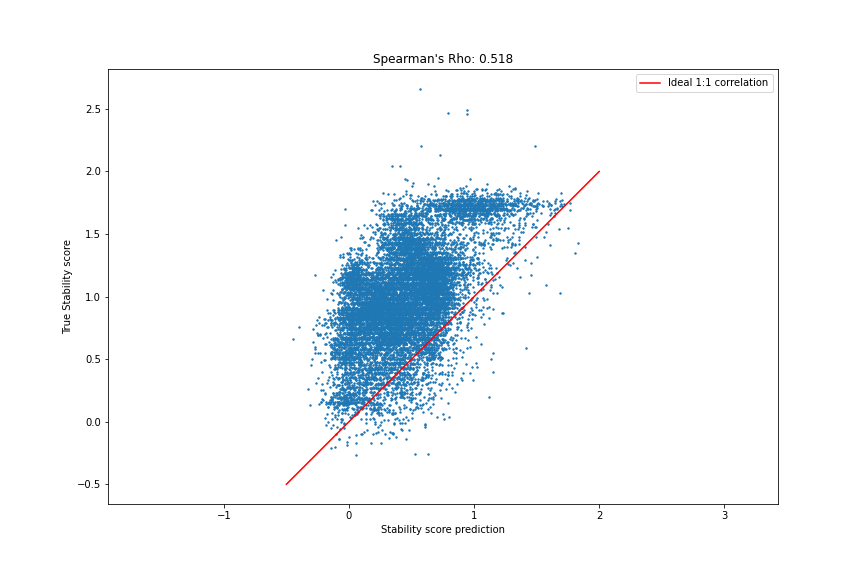
\includegraphics[width=0.49\linewidth]{latex/imgs/spearman_2_layer_05_drop_final.png}
  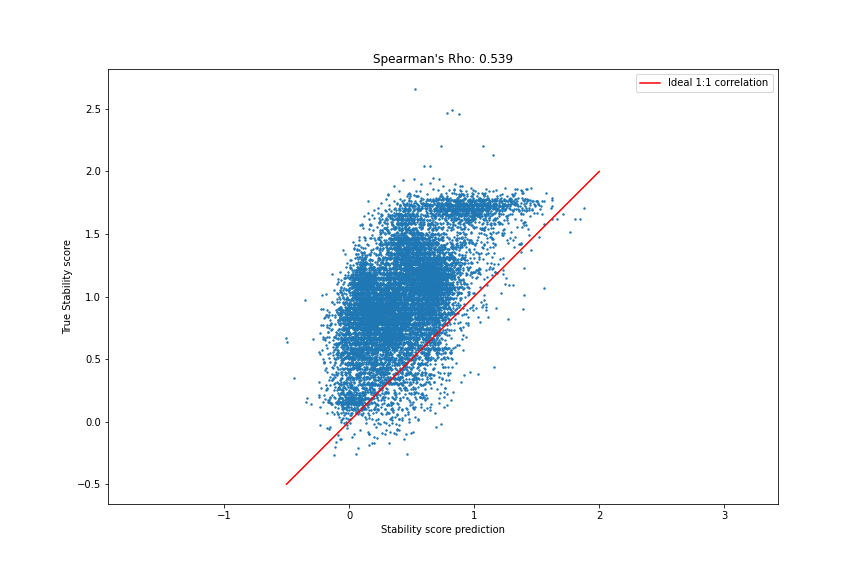
\includegraphics[width=0.49\linewidth]{latex/imgs/spearman_2_layer_05_drop_minloss.png}
  \caption{Final and minloss comparison of the Spearman's rho data plots of the 2-layer, $50\%$ dropout, $512$ feature model.}
\end{figure}
\begin{figure}[!ht]
  % 0.400 and 0.427
  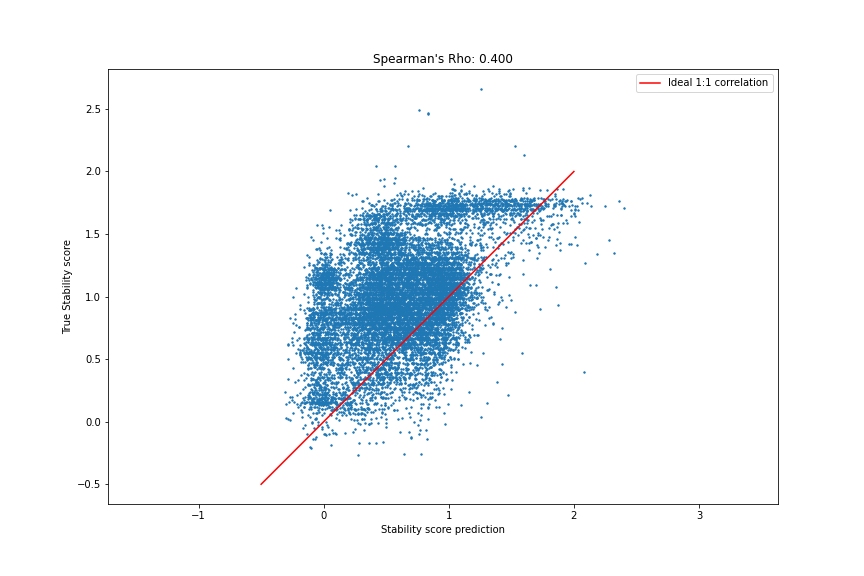
\includegraphics[width=0.49\linewidth]{latex/imgs/spearman_2_layer_no_drop_final.png}
  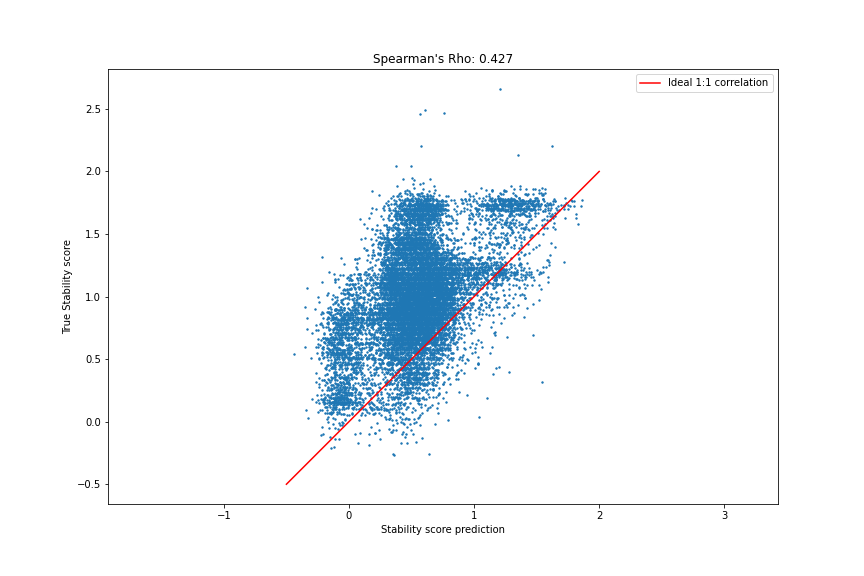
\includegraphics[width=0.49\linewidth]{latex/imgs/spearman_2_layer_no_drop_minloss.png}
  \caption{Final and minloss comparison of the Spearman's rho data plots of the 2-layer, no dropout, $512$ feature model.}
\end{figure}
\begin{figure}[!ht]
  % 0.605 and 0.592
  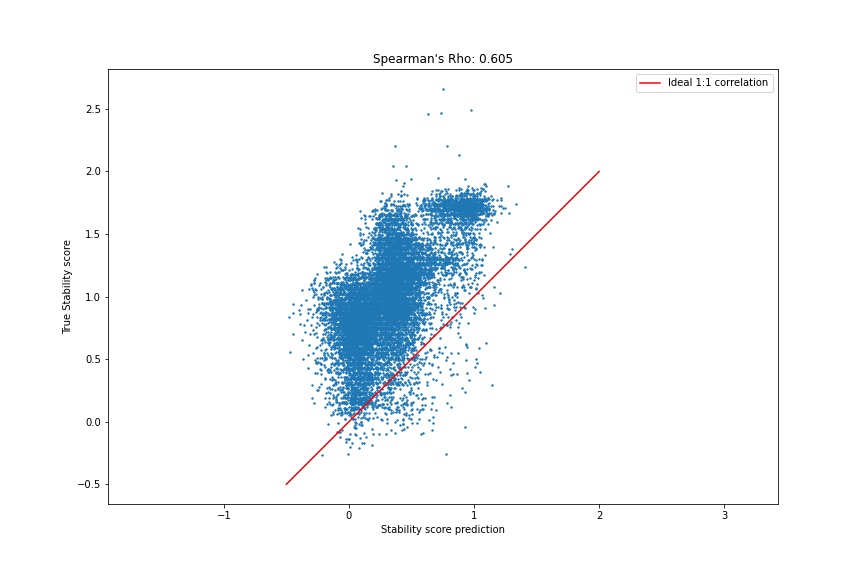
\includegraphics[width=0.49\linewidth]{latex/imgs/spearman_1_layer_no_schedule_512_final.png}
  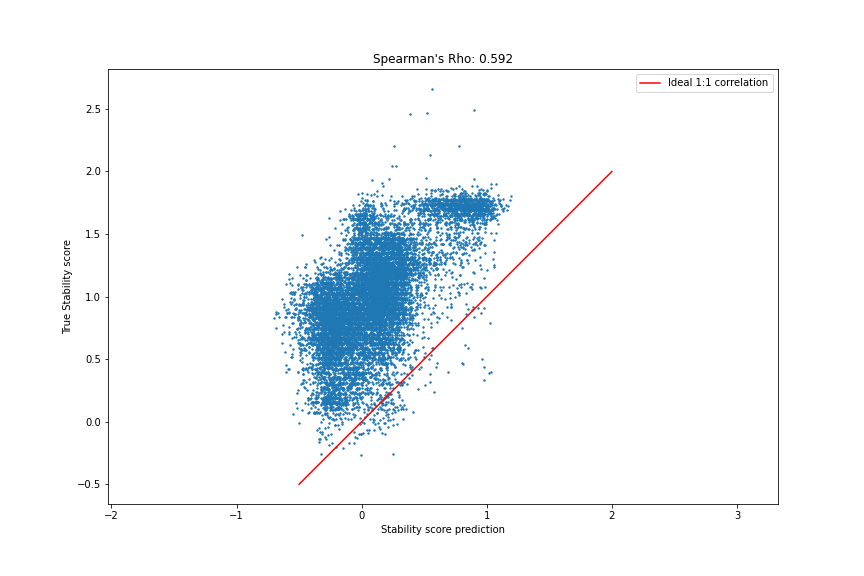
\includegraphics[width=0.49\linewidth]{latex/imgs/spearman_1_layer_no_schedule_512_minloss.png}
  \caption{Final and minloss comparison of the Spearman's rho data plots of the 1-layer, no lr schedule, $512$ feature model.}
\end{figure}
\begin{figure}[!ht]
  % 0.428 and 0.414
  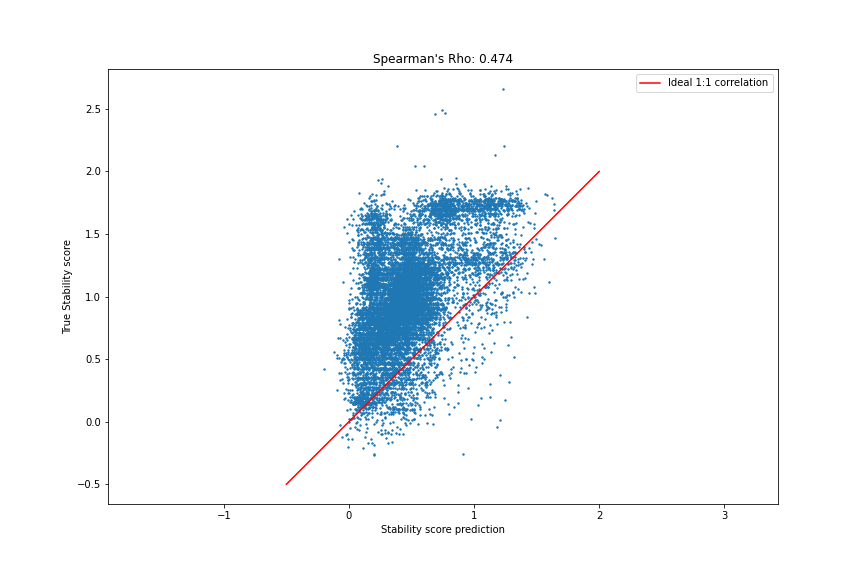
\includegraphics[width=0.49\linewidth]{latex/imgs/spearman_1_layer_with_schedule_512_final.png}
  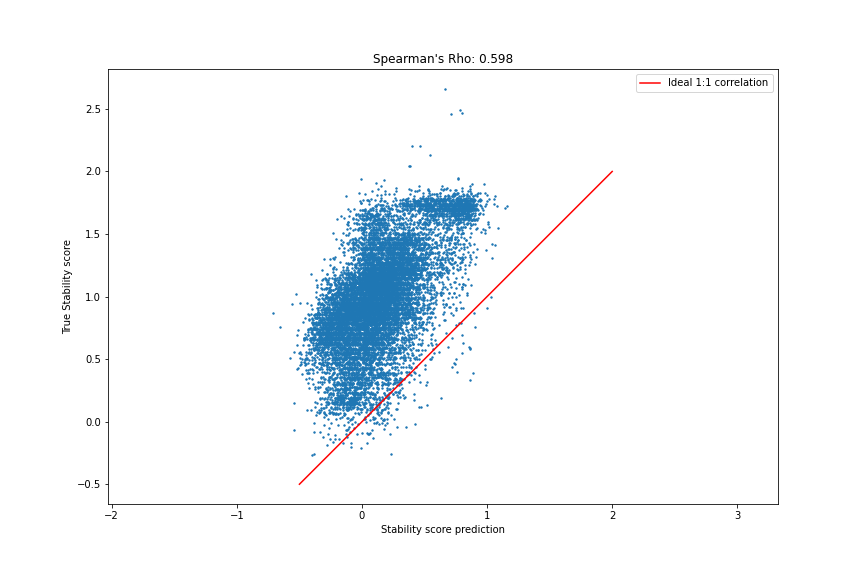
\includegraphics[width=0.49\linewidth]{latex/imgs/spearman_1_layer_with_schedule_512_minloss.png}
  \caption{Final and minloss comparison of the Spearman's rho data plots of the 1-layer, $512$ feature model.}
\end{figure}
\begin{figure}[!ht]
  % 0.435 and 0.424
  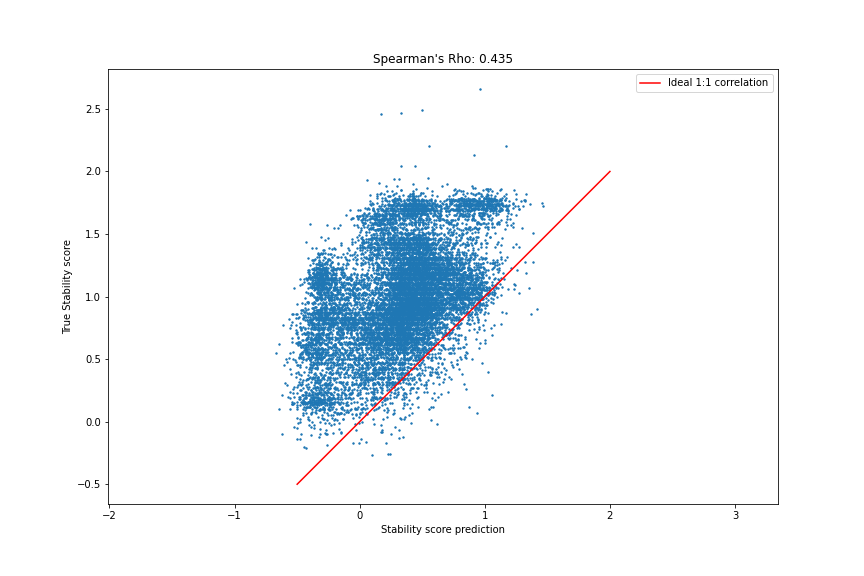
\includegraphics[width=0.49\linewidth]{latex/imgs/spearman_1_layer_with_schedule_256_final.png}
  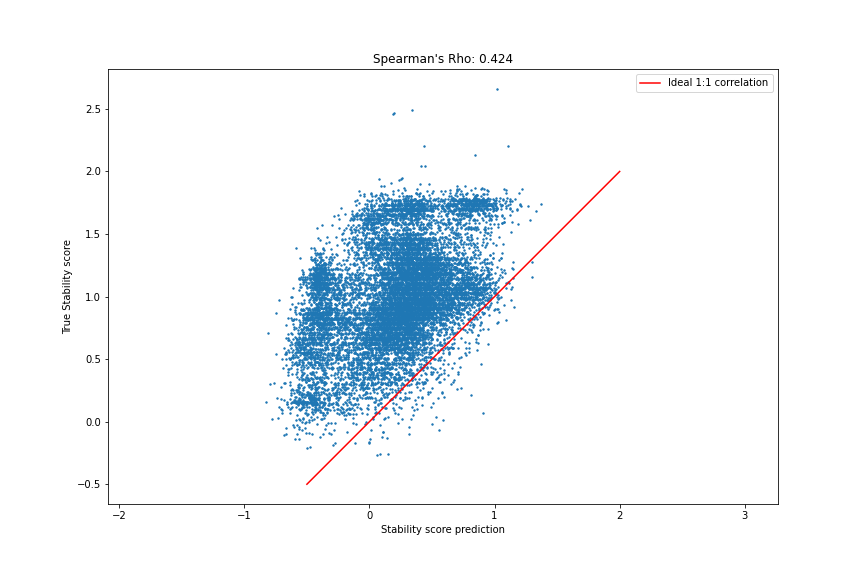
\includegraphics[width=0.49\linewidth]{latex/imgs/spearman_1_layer_with_schedule_256_minloss.png}
  \caption{Final and minloss comparison of the Spearman's rho data plots of the 1-layer, $256$ feature model.}
\end{figure}
\begin{figure}[!ht]
  % 0.507 and 0.627
  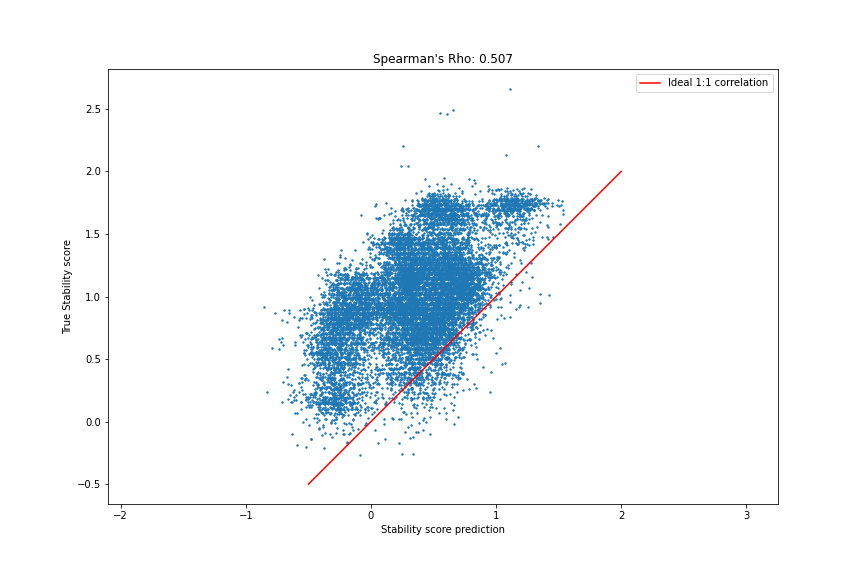
\includegraphics[width=0.49\linewidth]{latex/imgs/spearman_1_layer_with_schedule_1024_final.png}
  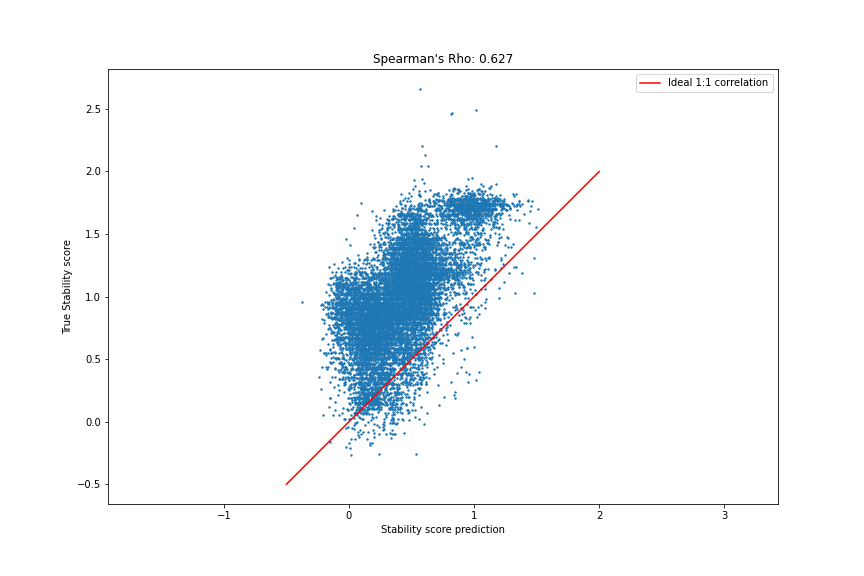
\includegraphics[width=0.49\linewidth]{latex/imgs/spearman_1_layer_with_schedule_1024_minloss.png}
  \caption{Final and minloss comparison of the Spearman's rho data plots of the 1-layer, $1024$ feature model.}
\end{figure}

%%%%%%%%%%%%%%%%%%%%%%%%%%%%
% TSNE
%%%%%%%%%%%%%%%%%%%%%%%%%%%%

\begin{figure}[!ht]
  \centering
  % 0.518 and 0.539
  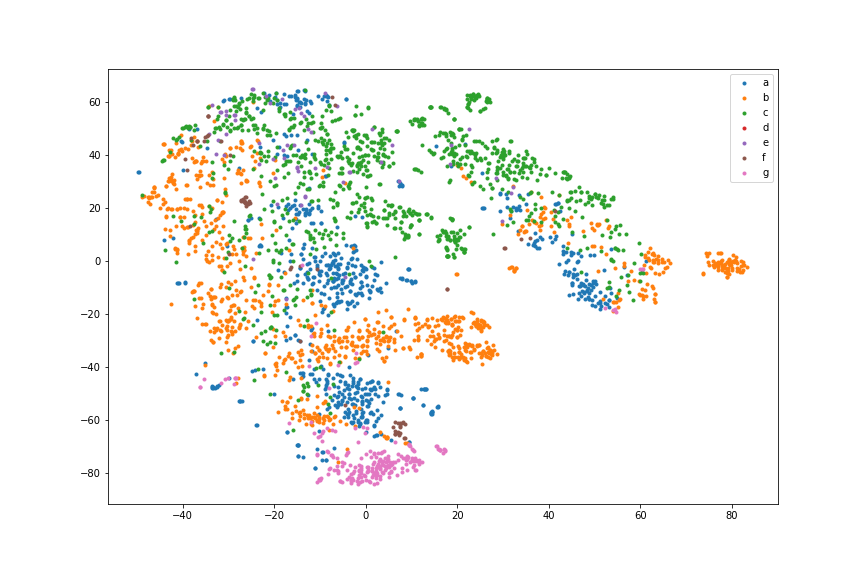
\includegraphics[width=0.49\linewidth]{latex/imgs/tsne_2_layer_05_drop_final.png}
  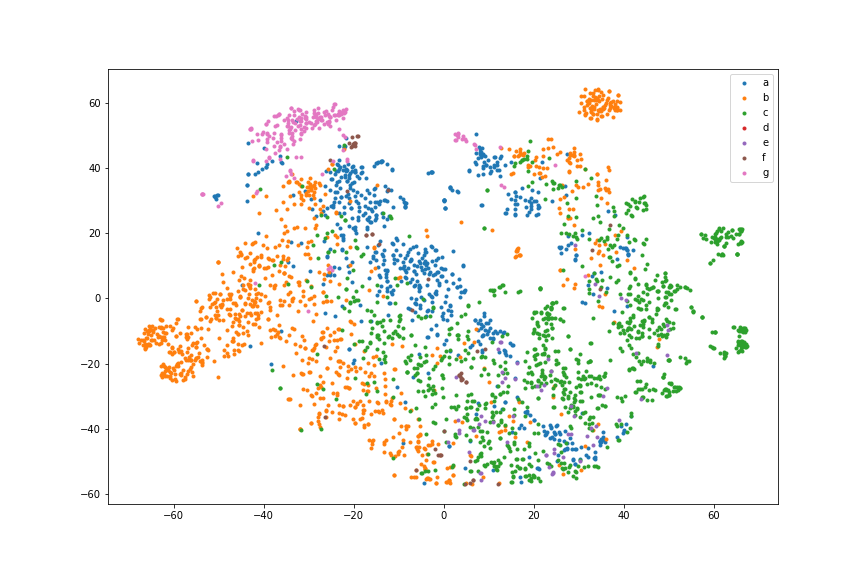
\includegraphics[width=0.49\linewidth]{latex/imgs/tsne_2_layer_05_drop_minloss.png}
  \caption{Final and minloss comparison of the TSNE dimensionality reduction plots of the 2-layer, $50\%$ dropout, $512$ feature model.}
\end{figure}
\begin{figure}[!ht]
  % 0.400 and 0.427
  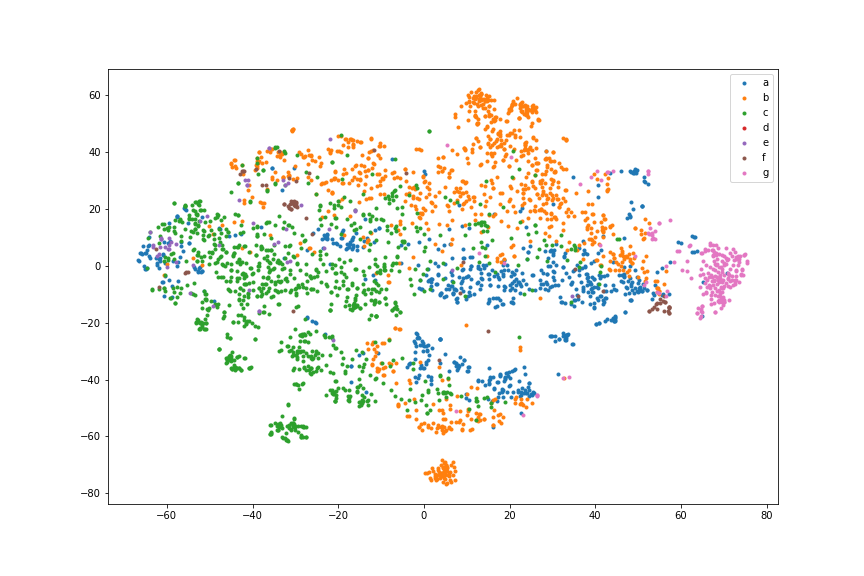
\includegraphics[width=0.49\linewidth]{latex/imgs/tsne_2_layer_no_drop_final.png}
  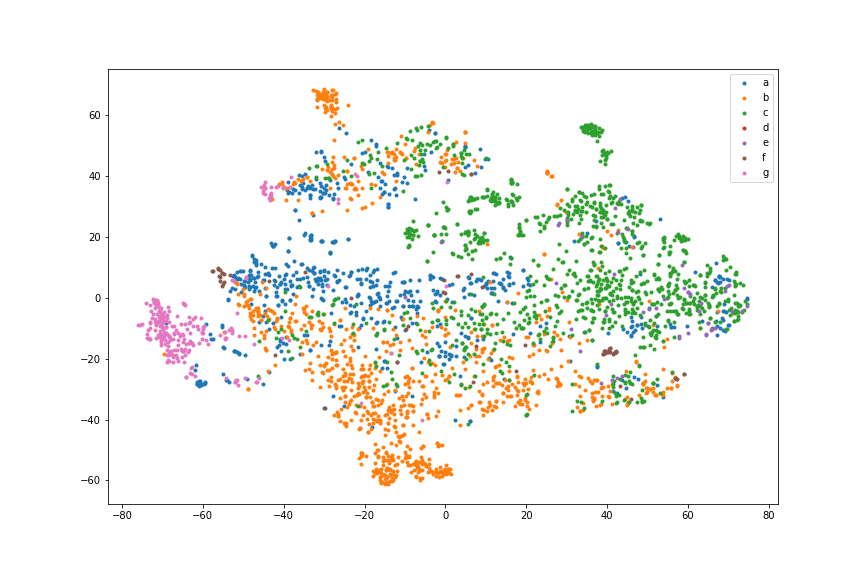
\includegraphics[width=0.49\linewidth]{latex/imgs/tsne_2_layer_no_drop_minloss.png}
  \caption{Final and minloss comparison of the TSNE dimensionality reduction plots of the 2-layer, no dropout, $512$ feature model.}
\end{figure}
\begin{figure}[!ht]
  % 0.605 and 0.592
  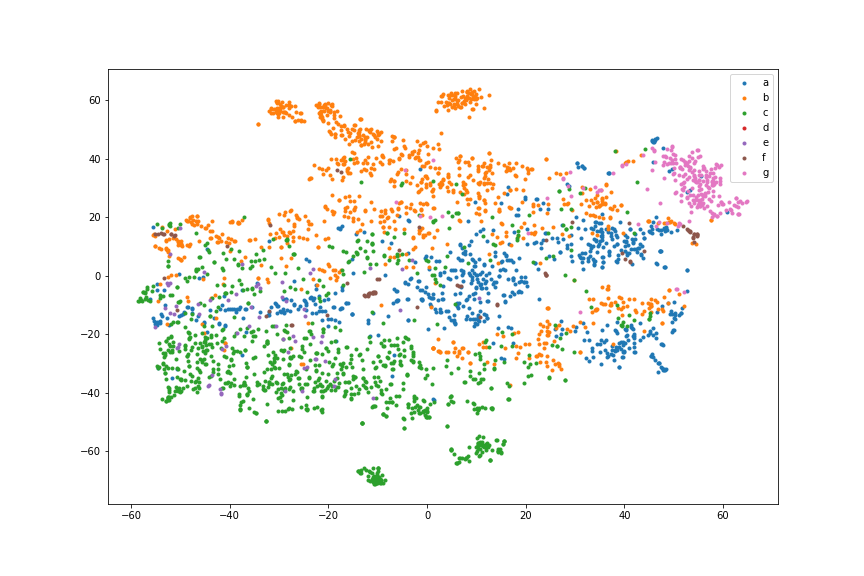
\includegraphics[width=0.49\linewidth]{latex/imgs/tsne_1_layer_no_schedule_512_final.png}
  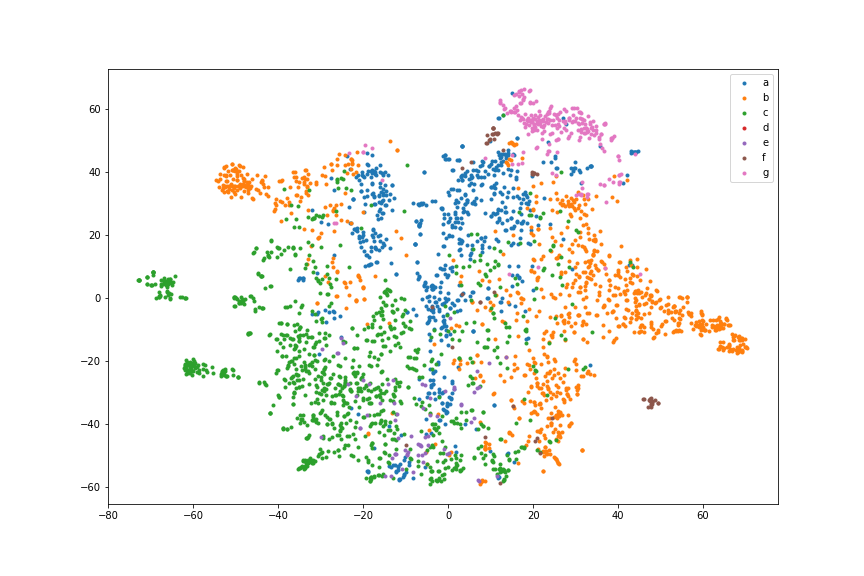
\includegraphics[width=0.49\linewidth]{latex/imgs/tsne_1_layer_no_schedule_512_minloss.png}
  \caption{Final and minloss comparison of the TSNE dimensionality reduction plots of the 1-layer, no lr schedule, $512$ feature model.}
\end{figure}
\begin{figure}[!ht]
  % 0.428 and 0.414
  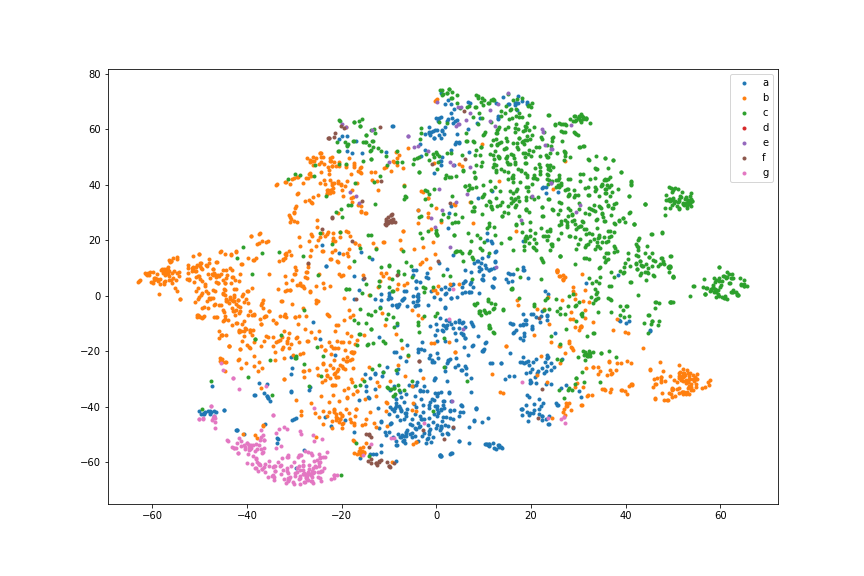
\includegraphics[width=0.49\linewidth]{latex/imgs/tsne_1_layer_with_schedule_512_final.png}
  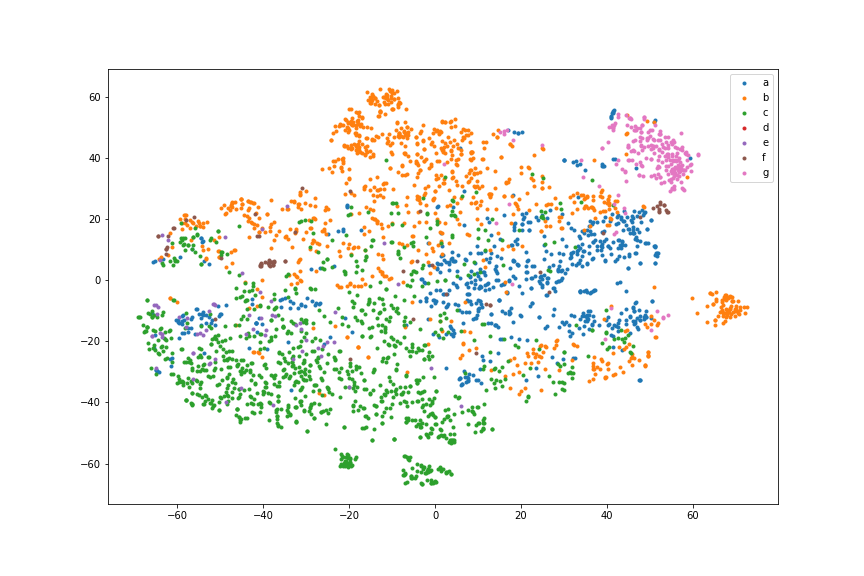
\includegraphics[width=0.49\linewidth]{latex/imgs/tsne_1_layer_with_schedule_512_minloss.png}
  \caption{Final and minloss comparison of the TSNE dimensionality reduction plots of the 1-layer, $512$ feature model.}
\end{figure}
\begin{figure}[!ht]
  % 0.435 and 0.424
  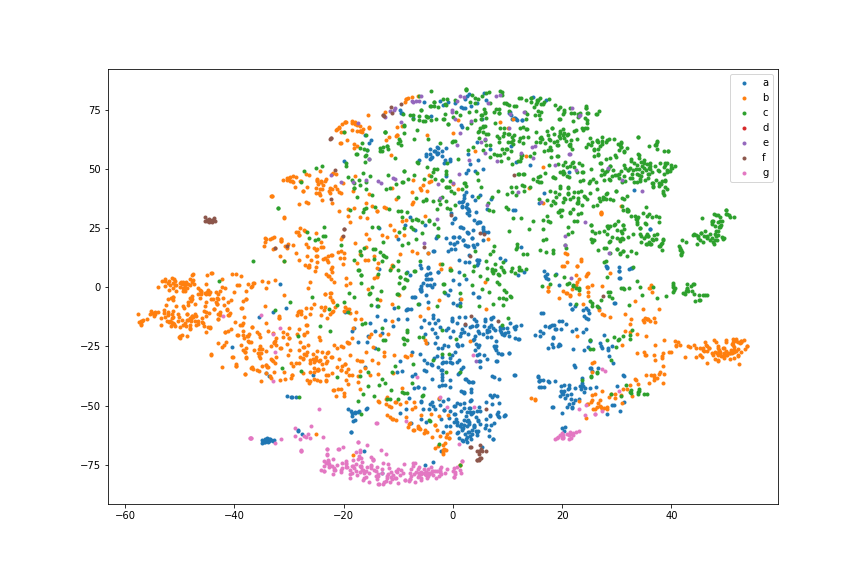
\includegraphics[width=0.49\linewidth]{latex/imgs/tsne_1_layer_with_schedule_256_final.png}
  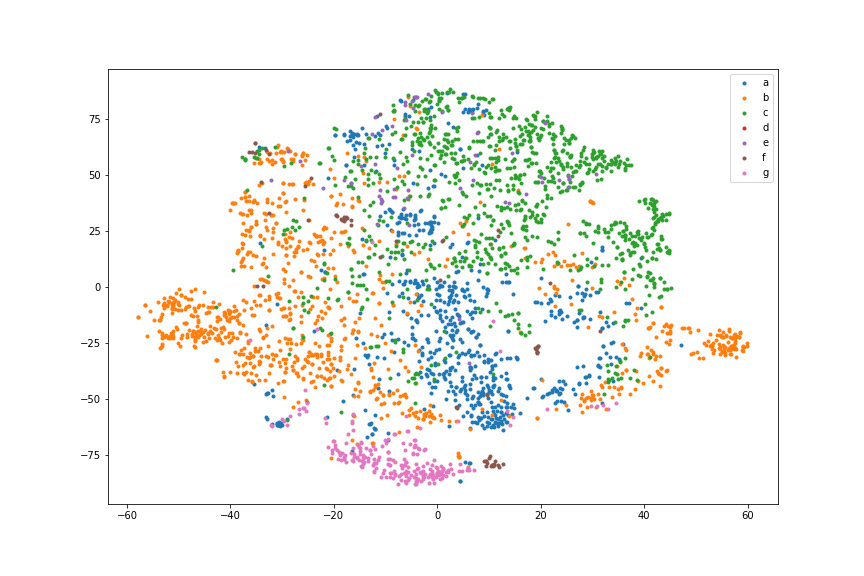
\includegraphics[width=0.49\linewidth]{latex/imgs/tsne_1_layer_with_schedule_256_minloss.png}
  \caption{Final and minloss comparison of the TSNE dimensionality reduction plots of the 1-layer, $256$ feature model.}
\end{figure}
\begin{figure}[!ht]
  % 0.507 and 0.627
  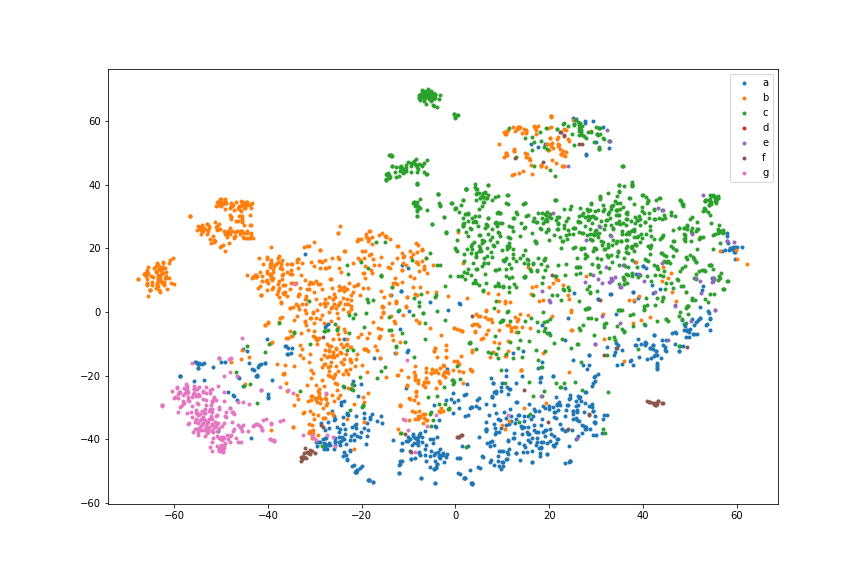
\includegraphics[width=0.49\linewidth]{latex/imgs/tsne_1_layer_with_schedule_1024_final.png}
  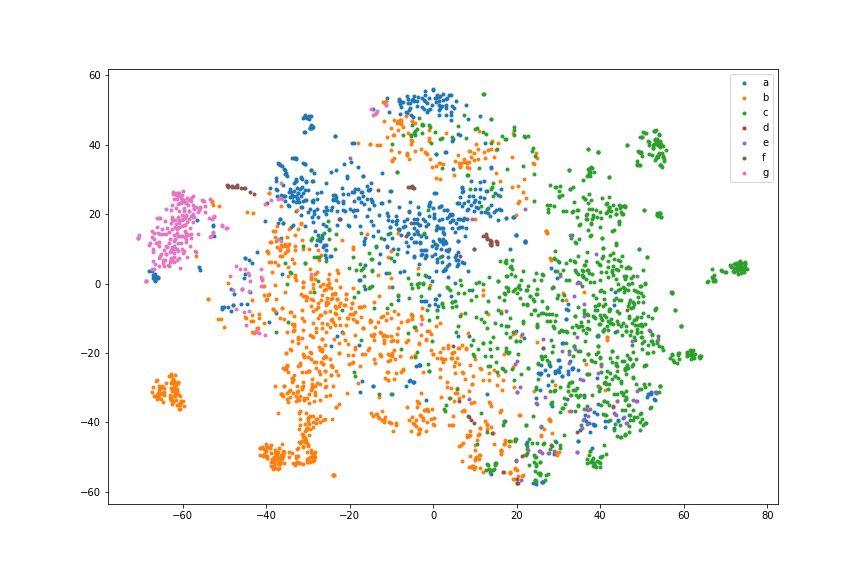
\includegraphics[width=0.49\linewidth]{latex/imgs/tsne_1_layer_with_schedule_1024_minloss.png}
  \caption{Final and minloss comparison of the TSNE dimensionality reduction plots of the 1-layer, $1024$ feature model.}
\end{figure}
